Whilst chemists frequently use the near and mid\nobreakdash-infrared (\acrshort{ir}) regions of the \acrfull{em} spectrum regularly in their research, the far\nobreakdash-\acrshort{ir} or terahertz (\acrshort{thz}) region, commonly defined as 0.1\nobreakdash--\SI{10}{\acrshort{thz}} or 3\nobreakdash--\DIFdelbegin %DIFDELCMD < \SI{333}{cm^{-1}}%%%
\DIFdelend \DIFaddbegin \SI{300}{cm^{-1}}\DIFaddend , has been comparatively underutilised. This was a result of the lack of coherent, strong sources of \acrshort{em} radiation in this frequency range, the so\nobreakdash-called `Terahertz Gap', and the location of this region between the microwave and \acrshort{ir} regions is shown in \Cref{fig:emspectrum}. For brevity, \acrshort{thz} \acrshort{em} radiation will be referred to as \acrshort{thz} radiation for the remainder of this document. In the previous decades, the technology behind sources and detectors for \acrshort{thz} radiation has seen significant improvements and this has resulted in a sharp increase in the number of studies that involve \acrshort{thz} radiation across a variety of applications \DIFdelbegin \DIFdel{~}\DIFdelend \cite{Lewis2014}. 

\begin{figure}
    \centering
    
\includegraphics[scale = 0.6]{Figures/Misc/Theory/EMSpectrum.png}
    \captionsetup{font = footnotesize, justification = centering}
    \caption[A Graphic of the Electromagnetic Spectrum]{A graphic of the EM spectrum indicating the relative position of the far-IR or \acrshort{thz} region with electronic and optical arrows indicating the traditional method of generation.}
    \label{fig:emspectrum}
\end{figure}

\section{Applications of Terahertz Radiation}
Owing to the nature of \acrshort{thz} radiation, it can penetrate most non\nobreakdash-conducting and non\nobreakdash-polar materials which can provide advantages over traditional visible and \acrshort{ir} based imaging systems, allowing for potential applications in security screening of both people \DIFdelbegin \DIFdel{~}\DIFdelend \cite{Appleby2007} and commercial packaging \DIFdelbegin \DIFdel{~}\DIFdelend \cite{Federici2005}.
Whilst \acrshort{thz} can transmit through these types of materials, it is severely attenuated by water which is a polar molecule. \acrshort{thz} radiation is also non\nobreakdash-ionising which means it can be used to image materials non\nobreakdash-destructively. These properties have led to the development of a number of biological and medical applications \DIFdelbegin \DIFdel{~}\DIFdelend \cite{Wu2019, Goretti2022, Chen2021, Osman2020, Ruan2019}.
\acrshort{thz} radiation's sensitivity to water content has been utilised for medical applications where highly sensitive measurements of water content can be used to differentiate between different tissue types \DIFdelbegin \DIFdel{~}\DIFdelend \cite{Bennett2011}. This may also be used for the detection and monitoring of certain types of cancer cells \DIFdelbegin \DIFdel{~}\DIFdelend \cite{Yu2012}. 
A significant commercial application of \acrshort{thz} imaging in the pharmaceutical industry has been the investigations into tablet coatings \DIFdelbegin \DIFdel{~}\DIFdelend \cite{Ho2008}. Until recently, the methods used to investigate tablets were generally destructive or were not suitable for on\nobreakdash-line rapid measurements \DIFdelbegin \DIFdel{~}\DIFdelend \cite{Mowery2002}. \acrfull{tpi} overcomes these issues as it is non\nobreakdash-destructive, sensitive to small changes in the refractive index of a material owing to reflections occurring at these interfaces and can suitably penetrate most pharmaceutically active compounds and common inert tablet components such as lactose. If the refractive index of the sample is known, these reflections can be utilised to extract accurate values for the thickness of each layer even in complex sample geometries. As the wavelength of \acrshort{thz} radiation is often longer than the particle size, scattering is minimal in these measurements compared to using conventional methods \DIFdelbegin \DIFdel{~}\DIFdelend \cite{Korasa2018}. Extremely thin layers (<~\SI{20}{\micro\metre}) are not suitably separated in the time\nobreakdash-domain, and so it has been shown that \acrshort{tpi} can be used in conjunction with other non-destructive imaging techniques such as Optical Coherence Tomography \DIFdelbegin \DIFdel{~}\DIFdelend \cite{Lin2017} to provide a complete picture of the geometry of these multi-layer systems. 

Whilst \acrshort{thz} imaging has seen significant improvements and has several important applications, the main focus and majority of technological development in this region of the \acrshort{em} spectrum has been on a branch of spectroscopy that has begun to come to maturity. This is called \acrfull{tds} and allows for the ability to probe the far\nobreakdash-\acrshort{ir} in a way that is not possible using traditional methods of generating \acrshort{ir} radiation. This is owing to the increasing power of \acrshort{thz} sources and a higher \acrfull{snr} in this region when compared to traditional \acrshort{ir} measurement methods such as \acrfull{ftir} in this lower frequency range. The raw signals produced by this technique are shown in \Cref{fig:exampletd} where it can be seen that the sample trace has been delayed and attenuated in comparison to the reference trace. These differences can be used to extract the frequency\nobreakdash-dependent absorption coefficient and refractive index of a sample, along with its real and complex permittivity \DIFdelbegin \DIFdel{~}\DIFdelend \cite{Burnett2016}. A more detailed discussion of \acrshort{tds} will be provided in \Cref{ch:exp_theory}.

\begin{figure}[t]
    \centering
    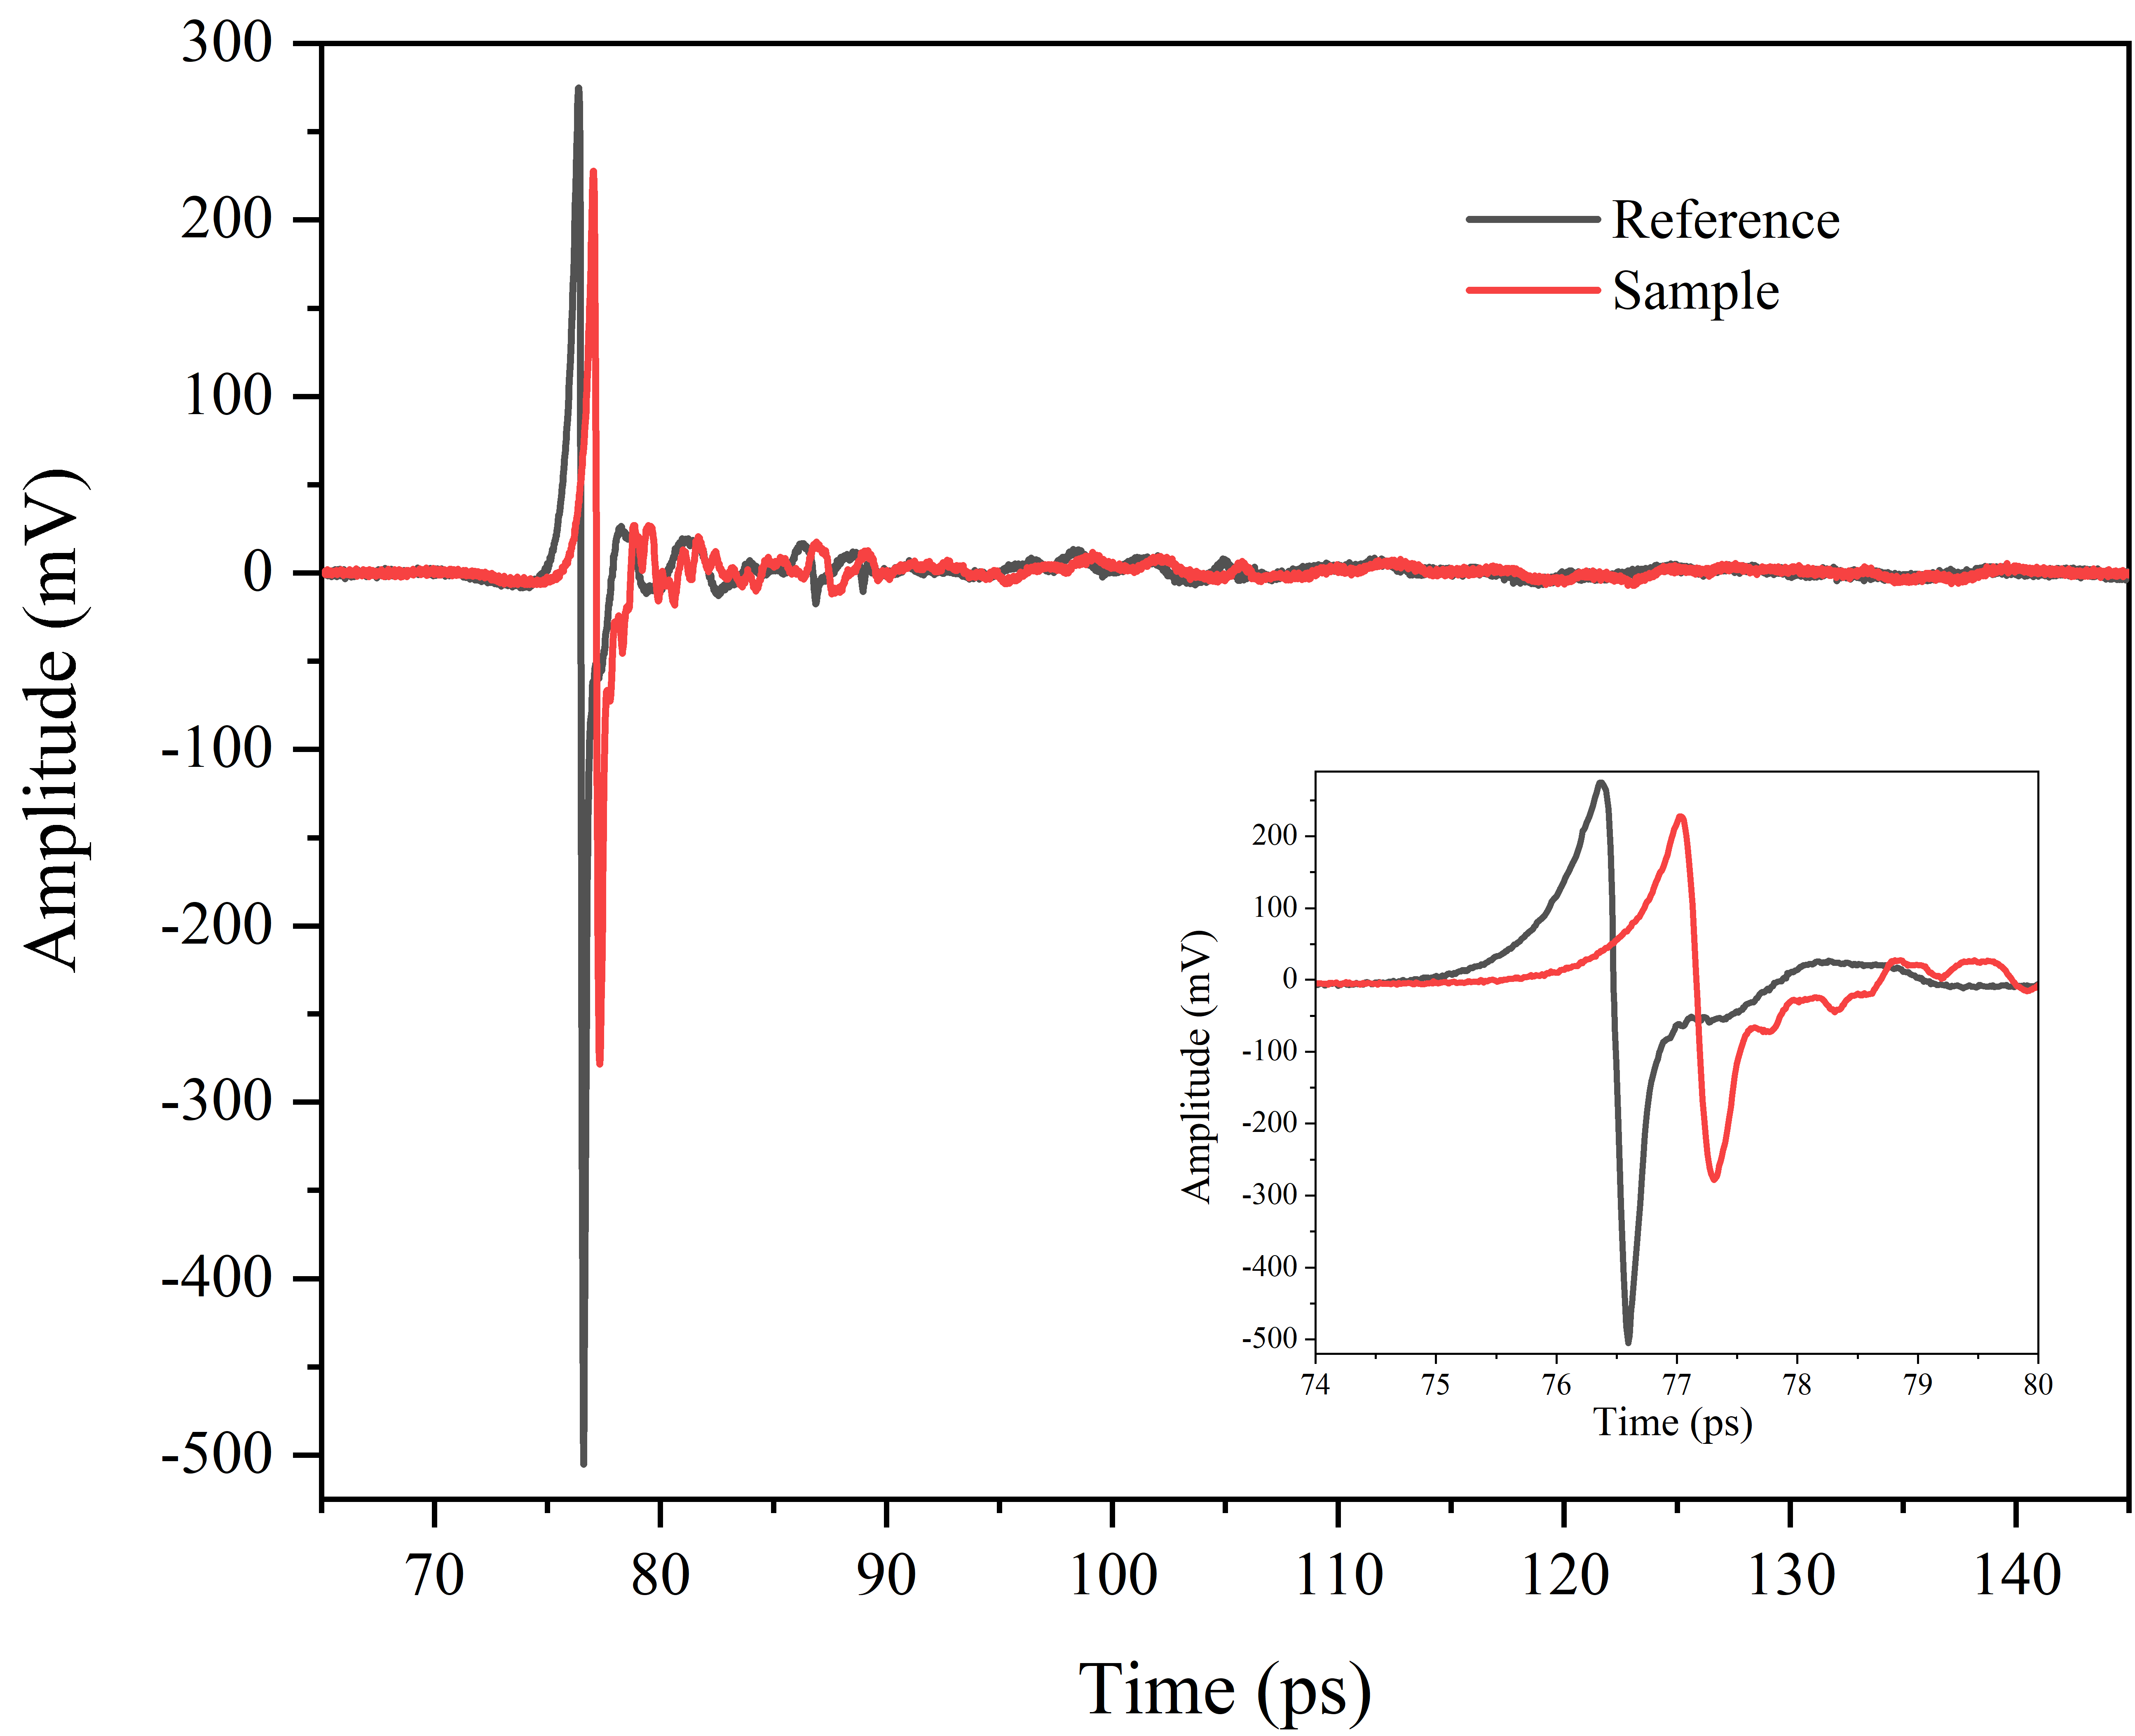
\includegraphics[scale=0.6]{Figures/Misc/Theory/TimeDomainFigureG.png}
    \captionsetup{font = footnotesize, justification = centering}
    \caption[A Sample and Reference Measurement in the Time Domain]{An example of two \acrshort{tds} scans, where one has a sample placed in the beam path and the other is dry air which is used as a reference. It can be seen that the trace that represents the sample has been attenuated and delayed in time. The inset shows the same two traces but with a focus on the main pulses.}
    \label{fig:exampletd}
\end{figure}

Whilst the mid\nobreakdash-\acrshort{ir} region corresponds to the frequency range of the vibrations of intra\nobreakdash-molecular bonds and the near\nobreakdash-\acrshort{ir} region contains the combination and overtone modes of these vibrations, the phenomena in the far\nobreakdash-\acrshort{ir} are much more challenging to interpret. 
Instead of the vibrations between atoms within a molecule, the motions in the far\nobreakdash-\acrshort{ir} consist of inter\nobreakdash-molecular vibrations, hindered rotations and torsions in the solid phase and free rotations in the gas phase. In the solid phase, these are extremely dependent on the surrounding long\nobreakdash-range ordering and overall chemical environment and are often referred to as phonons. Owing to the complex motions involved with these intermolecular modes, simple assignment linked to functional groups that occurs in the mid and near\nobreakdash-\acrshort{ir} is not possible and even clean, well resolved spectra of common organic materials can be challenging to interpret. This results in one of \acrshort{tds} greatest strengths, which is its sensitivity to minute changes in molecular and crystalline structure and their dynamics. However, this also increases the challenge of understanding the underlying phenomena without the aid of computational modelling of the chemical environment and comparison to experimental data. A detailed discussion of these computational methods and the modelling of vibrational properties of molecules and crystals will be provided in \Cref{ch:dft_theory}.

This sensitivity to the surrounding chemical environment can be utilised in a variety of ways. As even the smallest changes in this long\nobreakdash-range environment cause changes in the \acrshort{tds} spectrum, it can be a powerful tool for characterising drugs and their polymorphs \DIFdelbegin \DIFdel{~}\DIFdelend \cite{Wang2022}, even when \acrfull{xrd} is incapable of distinguishing between materials \DIFdelbegin \DIFdel{~}\DIFdelend \cite{Zeitler2016, Song2021, Druzbicki2015}. Several studies have also been done on the interaction of \acrshort{thz} radiation with amorphous materials and have found that \acrshort{thz} radiation can interact with the \acrfull{vdos}, the collective vibrational modes of non-crystalline materials. This has been shown to be useful as a probe for crystallisation, as sharp peaks begin to be identifiable on top of the broad absorption of the \acrshort{vdos} \DIFdelbegin \DIFdel{~}\DIFdelend \cite{Zeitler2007}. This broad absorption is owing to the strong dampening effect that a non\nobreakdash-crystalline structure has on intermolecular motions \DIFdelbegin \DIFdel{~}\DIFdelend \cite{Walther2003}. This can be useful as certain new drugs are only biologically active in their amorphous forms thus their shelf life is dependent of their rate of crystallisation \DIFdelbegin \DIFdel{~}\DIFdelend \cite{Shmool2019}. Owing to its non\nobreakdash-destructive nature and the drastic changes in the spectral features for chemically and structurally similar molecules, \acrshort{tds} radiation could potentially be used as a non-invasive way to detect dangerous materials in transport such as explosives or illegal drugs \DIFdelbegin \DIFdel{~}\DIFdelend \cite{Davies2008}.
\acrshort{thz} radiation is the appropriate energy to probe low energy inter\nobreakdash-molecular bonds such as H\nobreakdash-bond networks, in both liquids and solids, and their dynamics on the sub\nobreakdash-ps timescale. Owing to this interaction, liquid water absorbs \acrshort{thz} radiation, with two strong absorption bands at 650 and \SI{200}{cm^{-1}} respectively \DIFdelbegin \DIFdel{~}\DIFdelend \cite{Bellissent2016}. Whilst this can be a problem in most applications, it has allowed extensive study of water’s role in biological processes. Many of these studies have been done on the hydration shells and dynamics of a wide range of biomolecules \DIFdelbegin \DIFdel{~}\DIFdelend \cite{Laman2008}. Through the development of these studies, the role of water, has been upgraded in its importance in many biological processes including the molecular recognition of enzymes, and protein folding and denaturing \DIFdelbegin \DIFdel{~}\DIFdelend \cite{gompf2004}. Some more recent developments have continued to provide insight into nature of solvation processes in water \DIFdelbegin \DIFdel{~}\DIFdelend \cite{Stephens2022}. In water vapour there are a number of weakly absorbing modes throughout the  range \DIFdelbegin \DIFdel{~}\DIFdelend \cite{Slocum2013} and if these are not removed then spectral features can become obscured owing to the absorption peaks caused by the water vapour. Measurements taken in the \acrshort{thz} frequency range are first purged with dry air or dry nitrogen to prevent this. As mentioned above, the hydrogen bond networks of solids can also be probed by \acrshort{thz} radiation. This, alongside \acrshort{thz} radiation’s non\nobreakdash-destructive nature, is being utilised by the pharmaceutical industry to probe the nature of organic crystalline materials \DIFdelbegin \DIFdel{~}\DIFdelend \cite{Zhao2018}. 
\(k_BT\), which is the Boltzmann constant multiplied by the temperature, is the amount of energy available to an atom or molecule at a given temperature and determines what energy levels are available. The value of \(k_BT\) at room temperature corresponds to approximately \SI{6.21}{\acrshort{thz}}. This means that higher energy modes can be populated and molecules can move freely between energy states. These dynamics, including relaxation back to lower energy states and interaction between these modes, play a key role in a large proportion of chemical processes as these contribute significantly to the distribution of energy throughout a system \DIFdelbegin \DIFdel{~}\DIFdelend \cite{Ruggiero2016, Fujisaki2005}. Understanding these processes and the phenomena underlying them is key to furthering our understanding of material science. 

Most of the methods and applications above use \acrshort{thz} electric field strengths that cause linear interactions in the system of interest. However, owing to advancements in \acrshort{thz} generation efficiency, the electric field strengths have now become enough to induce non\nobreakdash-linear behaviour in various systems \DIFdelbegin \DIFdel{~}\DIFdelend \cite{Hwang2015}. The nature of these varies greatly, with non\nobreakdash-linear electrical carrier transport being one of the first non\nobreakdash-linear phenomena to be observed with \acrshort{thz} excitation \DIFdelbegin \DIFdel{~}\DIFdelend \cite{Ganichev2005}. Various groups have found non\nobreakdash-linear lattice effects in crystals \DIFdelbegin \DIFdel{~}\DIFdelend \cite{Hwang2015}, liquids \DIFdelbegin \DIFdel{~}\DIFdelend \cite{Hoffmann2009} and gases \DIFdelbegin \DIFdel{~}\DIFdelend \cite{Fleischer2012}, indicating that there are many more potential applications for \acrshort{thz} technologies as their generation efficiency and peak power increase. 

\section{Structure of Thesis and Aims of Project}
The thesis will begin with \Cref{ch:exp_theory} that will describe the theory behind the generation and detection of \acrshort{thz} \acrshort{em} radiation and how this is used in various measurement techniques, with a specific focus on \acrshort{tds}.

\Cref{ch:dft_theory} will begin with a mathematical description of vibrational modes and then examine the process behind modelling systems of interest using \acrfull{dft} and describe the methodology of calculating and interpreting a \acrshort{tds} spectrum.

\Cref{ch:ivdw} and \Cref{ch:qha} will be specifically focused on the further development of accurately modelling and analysing complex organic systems as this is one of the key challenges facing this technique. For this purpose, the molecule selected is \acrfull{alm}, shown in \Cref{fig:aLMbLMStructures}, owing to its sharp low-frequency features, particularly the peak at \SI{0.52}{\acrshort{thz}}/\SI{17}{cm^{-1}} which does not shift with temperature. \acrshort{alm} has recently been suggested to be an optimal candidate for a standard for both low\nobreakdash-frequency vibrational spectroscopy and the theoretical calculation of these spectra \DIFdelbegin \DIFdel{~}\DIFdelend \cite{Dampf2020}. \Cref{ch:ivdw} will compare the experimental \acrshort{thz} absorption spectrum, taken at \SI{4}{K}, to calculated \acrshort{thz} absorption spectra that have been obtained using five different dispersion corrections and attempt to provide a numerical justification for which is the most appropriate for organic systems and should be used moving forward.

 \begin{figure}[h]
\centering
\begin{subfigure}{0.49\textwidth}
\centering

\includegraphics[scale = 0.6]{Figures/Misc/Theory/aLM_structure.png}
\captionsetup{font = footnotesize, justification = centering}
\caption{The molecular structure of ${\alpha}$LM}
\label{fig:aLMStruct}
\end{subfigure}
\hfill
\begin{subfigure}{0.49\textwidth}
\centering

\includegraphics[scale = 0.6]{Figures/Misc/Theory/bLM_structure.png}
\captionsetup{font = footnotesize, justification = centering}
\caption{The molecular structure of ${\beta}$LM}
\label{fig:bLMStruct}
\end{subfigure}
\captionsetup{font = footnotesize, justification = centering}
\caption[The Molecular Structures of \(\alpha\) and \(\beta\) Lactose Monohydrate]{The molecular structures of \(\alpha\) and \(\beta\) Lactose Monohydrate. The asterisk marks the chirality centre on this molecule that determines which enantiomer is present.}
\label{fig:aLMbLMStructures}
\end{figure}

\Cref{ch:qha} will examine the effect of including structural anharmonicity into the calculation process with the aim of better modelling the system. This will be tested by attempting to produce a calculated room\nobreakdash-temperature spectrum and comparing this to experiment. Some thermodynamic properties, such as heat capacity, are also calculated in this process and these results are also discussed.

Finally, \Cref{ch:sys_dev} will examine the effect of the device gap size on photoconductive antennas used to generate \acrshort{thz} \acrshort{em} radiation on the produced radiation and its implications for future developments. There will then be some concluding remarks and suggestions for the next phases of the work done in this thesis.